\section{Introduction}
Isogeoemtric analysis (IGA) was introduced in 2005 by Hughes et al.~\cite{Hughes2005iac}, followed by the book~\cite{Cottrell2009iat} in 2009. Since then, IGA has received a great deal of attention in the effort of bridging the gap between finite element analysis (FEA) and computer aided design (CAD) tools. The initial problem that sparked the IGA movement was the cumbersome mesh generating process when converting the design models from CAD into the FEA programs, and the analysis could often imply a rerun of this tedious process. The problem being that the geometry is represented differently in CAD and FEA. 

An example is the geometries illustrated in \Cref{Fig3:NURBSexamples} which can be represented exactly using NURBS but is outside the space of standard (Lagrangian) FEM geometries.
\begin{figure}
	\centering
	\begin{subfigure}[b]{0.3\textwidth}
		\centering
		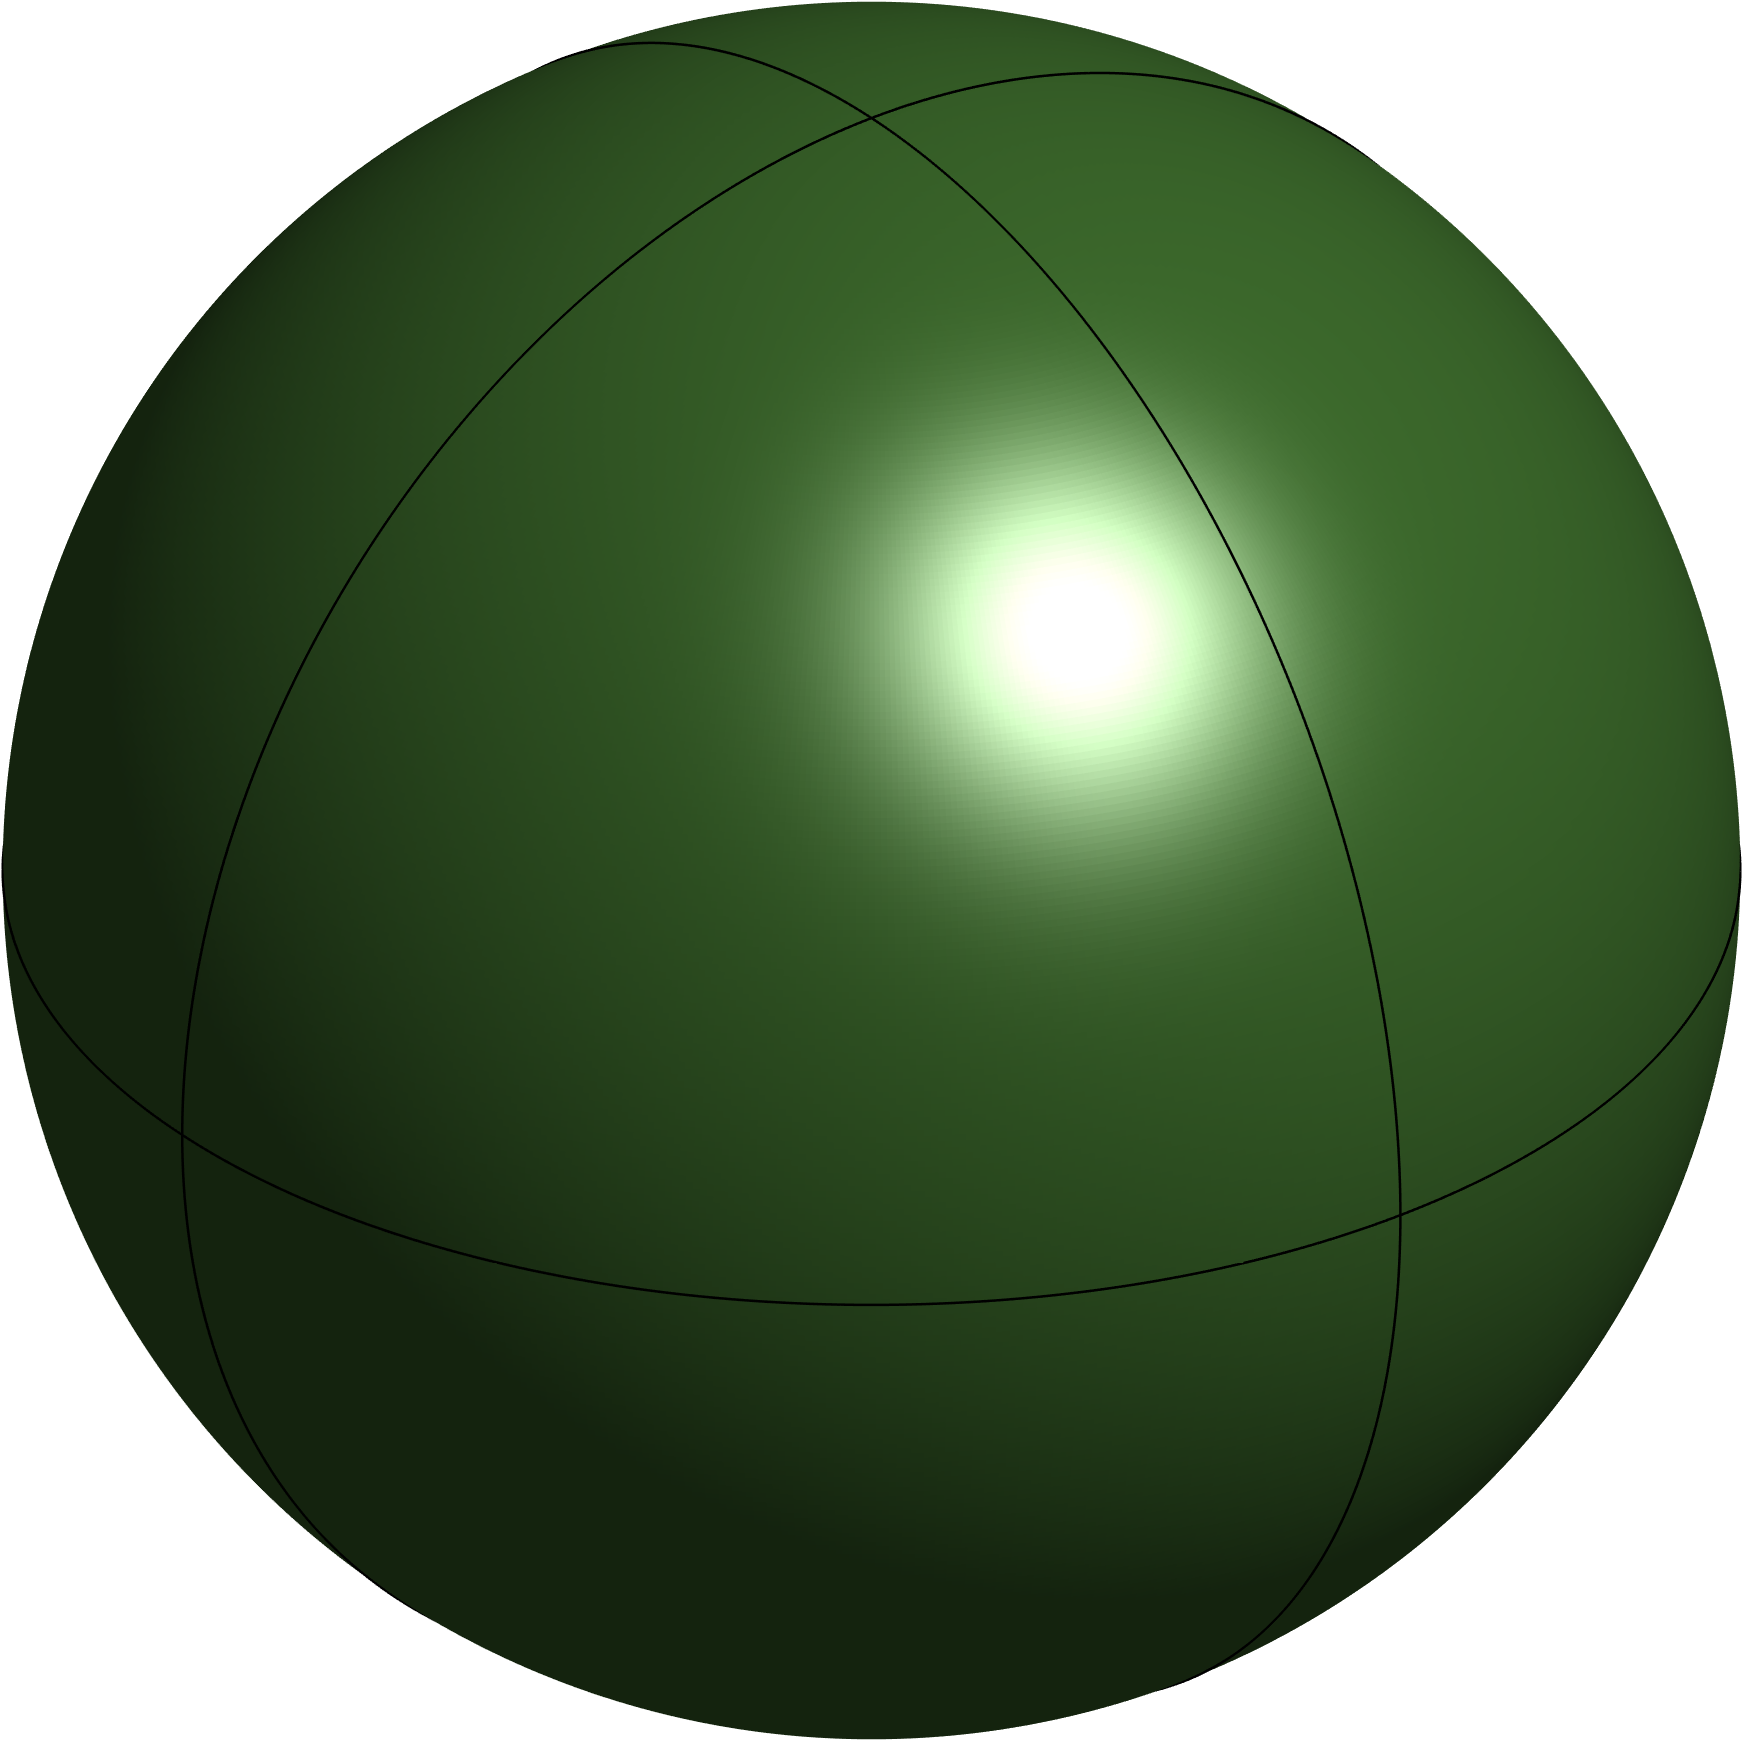
\includegraphics[width=0.9\textwidth]{../../graphics/sphericalShell/sphericalShellMesh1_2_0}
%		\includegraphics[width=0.9\textwidth]{\graphicsFolder/Figure1a}
		\caption{A sphere with 8 elements.}
		\label{Fig3:sphere}
	\end{subfigure}
	~    
	\begin{subfigure}[b]{0.35\textwidth}
		\centering
		\includegraphics[width=0.9\textwidth]{../../graphics/Torus}
%		\includegraphics[width=0.9\textwidth]{\graphicsFolder/Figure1b}
		\caption{A torus with 16 elements.}
		\label{Fig3:Torus}
	\end{subfigure}
	\caption{Examples of exact NURBS geometries of second degree.}
	\label{Fig3:NURBSexamples}
\end{figure} 
Using the same geometry representation as in CAD, IGA features exact geometry, which remains true in all mesh refinement procedures. Moreover, it turns out that using the non-uniform rational B-splines (NURBS) as basis functions not only for representing the geometry, but also the solution space, greatly enhances the numerical accuracy, see~\cite{BeiraodaVeiga2011sef} and~\cite{BeiraodaVeiga2014mao}. This motivates the use of IGA even further, as IGA enables control of the continuity of the basis function up to $C^{\check{p}-1}$ where $\check{p}$ is the polynomial degree (in contrast with the $C^0$-continuity restriction in classical FEA). 

For exterior problems, one can introduce an artificial boundary to obtain a bounded domain introducing the difficulty of surface-to-volume parametrization. The boundary element method (BEM) avoids this issue entirely as it only relies on a computational domain on the surface of the scatterer. Moreover, solid domains are usually represented by surfaces in CAD-systems, such that if modeling of an elastic scatterer is required, the BEM solves this problem as well without the need of surface-to-volume parametrization. This then represents an even further improvement of the quality of the design-analysis bridging development.

\begin{figure}
	\centering
	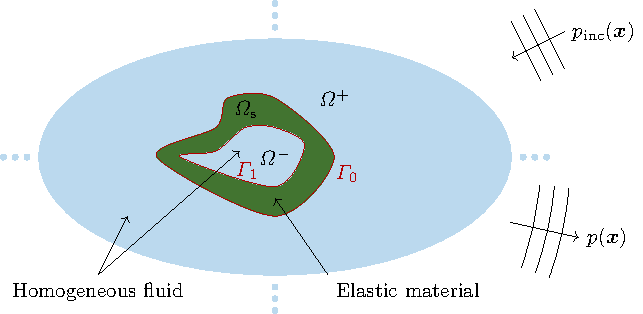
\includegraphics[scale=1]{../../LaTeX/createFigures/TikzFigures/articleBEM_PhD/physicalProblem}
%	\includegraphics[scale=1]{\graphicsFolder/Figure2}
	\caption{Illustration of the physical problem. A plane incident wave, $p_{\mathrm{inc}}(\vec{x})$, is scattered by the scatterer, represented by the closed boundary $\Gamma$, in an unbounded domain, $\Omega^+\subset\R^d$, resulting in the scattered pressure, $p(\vec{x})$.}
	\label{Fig3:physicalProblem}
\end{figure}
This work is only concerned with 3D acoustic scattering (with $d=3$). The main objective is scattering by plane waves, $p_{\rm inc}$, as illustrated in \Cref{Fig3:physicalProblem}. In scattering problems, it is often of interest to compute the target strength, $\TS$, of the scatterer in the far field. As an application of this work, the target strength is the quantity of interest for the acoustical aspects of constructing a submarine and is for this reason investigated in this work.

Assuming harmonic time dependency, all time dependent functions may be written as $\breve{F}=\breve{F}(\vec{x},t) = F(\vec{x})\euler^{-\imag\omega t}$ where $\omega$ is the angular frequency and $\imag = \sqrt{-1}$ the imaginary unit. This enables us to model the pressure $p$ in the fluid with the Helmholtz equation given by
\begin{equation}\label{Eq3:HelmholtzEquationIntro}
	\nabla^2 p + k^2 p = 0
\end{equation}
with the wave number $k=\frac{\omega}{c_{\mathrm{f}}}$ (where $c_{\mathrm{f}}$ is the wave speed in the fluid\footnote{Throughout this work we shall use $c_{\mathrm{f}}=\SI{1500}{m/s}$.}). Other important quantities include the frequency $f=\frac{\omega}{2\PI}$ and the wavelength $\lambda = \frac{2\PI}{k}$.

Some literature already exists for solving acoustic problems using IGABEM including \cite{Simpson2014aib,Keuchel2017eoh,Peake2013eib,Peake2014eai,Peake2015eib,Coox2017aii, Taus2015iaf,Dolz2016aib,Dolz2018afi,Sun2019dib,Wu2020iib}. Arguably there is a lack of work in the approximability for IGABEM simulations for more complex geometries, and one of the aims of this work is to contribute to fill this gap.

The exterior Helmholtz problem is presented in \Cref{Sec3:exteriorHelmholtz}, and the corresponding boundary integral equations are given in \Cref{Sec3:BIE}. Discretization of these integral equations either with the use of collocation or a Galerkin approach yields the boundary element method which is presented in \Cref{Sec3:BEM}. The weakly singular boundary integral equation requires care when using numerical quadrature and is discussed in \Cref{Sec3:numericalQuad}. In \Cref{Sec3:resultsDisc} the results for several benchmark problems are presented. Not only are these benchmark problems important in bug testing for code development, but it is also important to establish reliable results for a several geometries ranging in complexity. Finally, conclusions and suggested future work can be found in \Cref{Sec3:conclusions}. 

